
\chapter{Bidirectional Radiance Caching}
\label{chap:bidirectional_caching}

\section{A General Theoretical Framework for Radiance Caching}
Before proposing new radiance caching techniques, I first want to take a step back and formulate a theoretical backbone.
Radiance caching generally can be broken down into four steps:
\begin{enumerate}
    \item \textbf{Training}
    \begin{enumerate}
        \item \textbf{Query Prediction} First, we want to predict potential queries $\hat{q} = (\vec{x}, \vec{\omega}_o)$ according to a distribution $\hat{Q}(\hat{q})$.
        \item \textbf{Radiance Estimation} Given a predicted query $\hat{q}$, we want to estimate the outgoing radiance $L_o(\hat{q})$ at that query.
        For this, we can use any possible combination of radiance estimation techniques, such as path tracing, light tracing, photon mapping or bidirectional path tracing.
    \end{enumerate}
    \item \textbf{Inference}
    \begin{enumerate}
        \item \textbf{Query Sampling} We sample queries $q = (\vec{x}, \vec{\omega}_o)$ according to a distribution $Q(q)$.
        \item \textbf{Interpolation} Given a query $q$, we want to approximate the outgoing radiance $\hat{L}_o(q)$ by interpolating the radiance estimates of spatio-temporally nearby query predictions $\hat{q}$.
        We can use any storing and interpolation technique for this, such as nearest neighbor, linear interpolation or, in our case, the NRC.
        Note however, that this step generally introduces \emph{bias}.
    \end{enumerate}
\end{enumerate}

\paragraph{Cache Efficiency}
\label{par:cache_efficiency}
Using this framework we can observe that the \emph{cache efficiency} is optimal if the query prediction distribution $\hat{Q}(\hat{q})$ is equal to the query sampling distribution $Q(q)$.
Conversely, if we sample a query $q^*$ that can not be predicted by the query predictor (i.e. $\hat{Q}(q^*)=0$), we introduce fundamental bias into the radiance cache $\hat{L}_o(q^*)$, because the radiance cache will not contain an accurate radiance estimate for that query.
This happens, whenever the support of the query sampling distribution $Q$ is not contained in the support of the query prediction distribution $\hat{Q}$, i.e. $\supp(Q) \not\subseteq \supp(\hat{Q})$.

In the original formulation of radiance caching by \textcite{ward1988} and in NRC by \textcite{muller2021}, the filling of the cache and the querying are closely linked.
By decoupling these two steps, however, we gain a lot of flexibility in choosing different strategies for both steps.
The general idea of decoupling radiance estimation and visualization was already explored by others, notably \textcite{walter1999} and \textcite{tole2002}.

\section{The Path Space Integral Formulation}
\label{sec:path_space_integral}
To be able to robustly derive the following radiance estimators, we will use an alternative but equivalent formulation of the rendering equation as an integral over the path space, which was introduced by \textcite{veach1997}.
\begin{figure}[htb!]
    \centering
    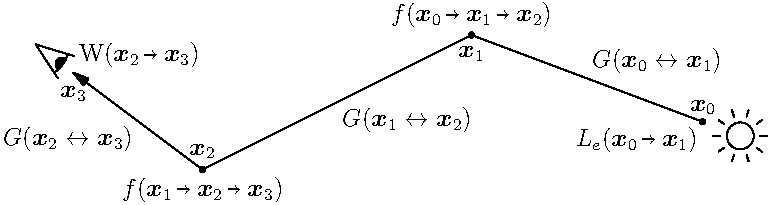
\includegraphics{asy/path_integral.pdf}
\caption{Radiance transfer along a path of length $n=3$ according to the path space integral formulation.}
\label{fig:path_space_integral}
\end{figure}

A path $\bar{x}$ of length $n$ is defined as a sequence of vertices $\vec{x}_0 \vec{x}_1 \cdots \vec{x}_n$.
Let the space of all paths of length $n$ be $X_n$ and the space of all paths $X = \bigcup_{n=1}^{\infty} X_n$.
Then, the path space integral formulation of the rendering equation is given by:
\begin{equation}
\label{eq:path_space_integral}
\begin{aligned}
    I
    = \sum_{n=0}^{\infty} \int_{X_n} L_e(\pdir{0}{1}) \G{0}{1} &\prod_{i=1}^{n - 1} \f{i-1}{i}{i+1} \G{i}{i+1}\\
    &\cdot W(\pdir{n-1}{n}) \diff A(\vec{x}_0) \cdots \diff A(\vec{x}_n)
\end{aligned}
\end{equation}
To collect incoming radiance at a sensor point $\vec{x}_n$, the path space integral formulation contains a sensor weighting term $W(\pdir{n-1}{n})$, which in the case of an infinitesimal pin-hole camera is simply a Dirac-Delta-function over the eye position and a box function over the viewing directions covered by the pixel.
The arrow notation $\vec{x} \pto \vec{y}$ denotes a ray starting at $\vec{x}$ traveling towards $\vec{y}$, i.e. $L_o(\vec{x} \pto \vec{y}) \defeq L_o(\vec{x}, \vec{y} - \vec{x})$.
The triples represent surface interactions, $f(\vec{x} \pto \vec{y} \pto \vec{z}) \defeq f(\vec{y} - \vec{x}, \vec{y}, \vec{z} - \vec{y})$. 
Double arrow notation is used for path segments, $G(\vec{x} \leftrightarrow \vec{y})$ models the radiance transfer between the vertices $\vec{x}$ and $\vec{y}$:
\begin{equation}
    \label{eq:transfer}
    G(\vec{x} \leftrightarrow \vec{y}) \defeq V(\vec{x} \leftrightarrow \vec{y}) \frac{\cos \theta_{\vec{x} \veryshortarrow \vec{y}} \cos \theta_{\vec{y} \veryshortarrow \vec{x}}}{\|\vec{y} - \vec{x}\|^2},
\end{equation}
where $V(\vec{x} \leftrightarrow \vec{y}) \in \{0,1\}$ defines visibility and $\theta$ denotes the respective angles of incidence.
The integral is measured over the surface of the scene $A(\vec{x})$.

\begin{figure}[htb!]
    \centering
    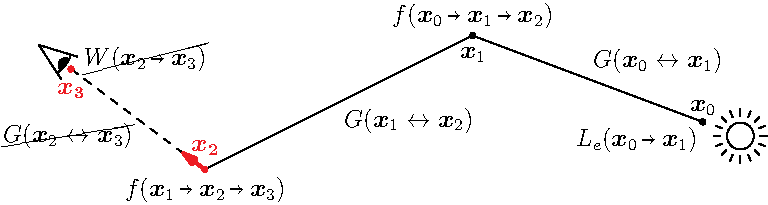
\includegraphics{asy/path_integral_radiance.pdf}
    \caption{To estimate the outgoing radiance $L_o(\pdir{2}{3})$ with the path space integral formulation, we fix the last two vertices defining the position and direction, here $\vec{x}_2$ and $\vec{x}_3$ highlighted in red. Furthermore, we drop the sensor weighting term $W$ and the last geometry term $\G{2}{3}$, because they are not part of the path anymore.}
    \label{fig:path_space_integral_radiance}
\end{figure}
In the following derivations, I will also use a slightly adapted formulation of the path space integral, that estimates \emph{radiance} instead of \emph{intensity} (see \cref{fig:path_space_integral_radiance}).
Therefore, we only have to drop the sensor weighting term $W$ and the last geometry term $\G{n-1}{n}$ and fix the last two vertices, which define the position and direction of outgoing radiance, by excluding them from the integration domain:
\begin{equation}
\label{eq:path_space_integral_radiance}
\begin{aligned}
    % L_o(x, \wo) = \sum_{n=0}^{\infty} \int_{X_n} L_e(\pdir{0}{1}) \G{0}{1} \prod_{i=1}^{n - 1} \f{i-1}{i}{i+1} \G{i}{i+1}\\
    % \f{n-1}{n}{} \G{n}{} f(\vec{x}_n \pto \vec{x}, \wo) \ \diff A(\vec{x}_0) \dots \diff A(\vec{x}_n)
    L_o(\pdir{n-1}{n})
    %= L_i(\pdir{n-1}{n})
    = &\sum_{n=0}^{\infty} \int_{X_{n-2}} L_e(\pdir{0}{1}) \\
    &\cdot \prod_{i=1}^{n - 1} \G{i-1}{i} \f{i-1}{i}{i+1} 
    \diff A(\vec{x}_0) \dots \diff A(\vec{x}_{n-2})
\end{aligned}
\end{equation}

The main advantage of these formulations is the independence of the individual vertices.
This for example allows for straightforward bidirectional sampling.
An essential tool for the derivation of path samplers is the conversion between area and solid angle measure, given by:
\begin{equation}
\label{eq:area_solid_angle}
    \diff \omega(\vec{x}\pto\vec{y}) = \frac{\cos \theta_{\vec{y}\veryshortarrow\vec{x}}}{\|\vec{y} - \vec{x}\|^2} \diff A(\vec{y}),
\end{equation}
or applied to sampling probabilities:
\begin{equation}
\label{eq:area_solid_angle_p}
    p(\vec{y}) \diff A(\vec{y}) = p(\vec{x}\pto\vec{y}) \diff \omega(\vec{x}\pto\vec{y}) \implies
    p(\vec{y})
    = \left| \frac{\diff \omega(\vec{x}\pto\vec{y})}{\diff A(\vec{y})}\right| p(\vec{x}\pto\vec{y})
    = \frac{\cos \theta_{\vec{y}\veryshortarrow\vec{x}}}{\|\vec{y} - \vec{x}\|^2} p(\vec{x}\pto\vec{y}).
\end{equation}

\section{Inference}
\label{sec:inference}
Using this framework a simple inference scheme naturally emerges from the Path Space Integral Formulation (\cref{eq:path_space_integral}).
The path length $n$ is limited by a path termination strategy (\cref{sec:path_termination}), so we only need to calculate the finite sum up to the termination length $l$ because we terminate with a valid radiance estimate which incorporates the sum over longer paths.
We replace the integral over the path space $X_n$ by a single-sample Monte-Carlo Estimator.
For readability, I will do an exemplary derivation for a path of length $n=2$ without intermediate emission:
\begin{subequations}
\begin{align}
    % Length n=2
    I
    &= \int_{X_n} \widehat{L}_o(\pdir{0}{1}) \G{0}{1} \f{0}{1}{2} \G{1}{2} \cancel{W(\pdir{1}{2})} \diff A(\vec{x}_0) \!\cdots\! \cancel{\diff A(\vec{x}_2)}\notag\\
    &= \int_{X_{n-1}} \widehat{L}_o(\pdir{0}{1}) \G{0}{1} \f{0}{1}{2} \G{1}{2} \diff A(\vec{x}_0) \diff A(\vec{x}_1) \label{eq:cancelw}\\
    &\eqhat \frac{\widehat{L}_o(\pdir{0}{1}) \G{0}{1}}{p(x_0)}  \frac{\f{0}{1}{2} \G{1}{2}}{p(x_1)} \label{eq:pmc}\\
    &= \frac{\widehat{L}_o(\pdir{0}{1}) \cos\theta_{1\veryshortarrow0}}{p(\pdir{1}{0}\mid\pdir{2}{1})}  \frac{\f{0}{1}{2} \cos\theta_{2\veryshortarrow1}}{p(\pdir{2}{1})} \label{eq:area2solid}
    % Length n=3
    % I
    % &= \int_{X_n} \widehat{L}_o(\pdir{0}{1}) \G{0}{1} \f{0}{1}{2} \G{1}{2} \f{1}{2}{3} \G{2}{3}  \cancel{W(\pdir{2}{3})} \diff A(\vec{x}_0) \cdots \cancel{\diff A(\vec{x}_3)}\\
    % &= \int_{X_{n-1}} \widehat{L}_o(\pdir{0}{1}) \G{0}{1} \f{0}{1}{2} \G{1}{2} \f{1}{2}{3} \G{2}{3} \diff A(\vec{x}_0) \cdots \diff A(\vec{x}_2)\\
    % &\eqhat \frac{\widehat{L}_o(\pdir{0}{1}) \G{0}{1}}{p(x_0)}  \frac{\f{0}{1}{2} \G{1}{2}}{p(x_1)} \frac{\f{1}{2}{3} \G{2}{3}}{p(x_2)}\\
    % &= \frac{\widehat{L}_o(\pdir{0}{1}) \cos\theta_{0\veryshortarrow1}}{p(\pdir{1}{0}\mid\pdir{2}{1})}  \frac{\f{0}{1}{2} \cos\theta_{1\veryshortarrow2}}{p(\pdir{2}{1}\mid\pdir{3}{2})} \frac{\f{1}{2}{3} \cos\theta_{2\veryshortarrow3}}{p(\pdir{3}{2})}\\
\end{align} % TODO: Make generic
\end{subequations}
In the first step, the sensor weighting term $W$ cancels with the integration over the eye vertex (\cref{eq:cancelw}).
We then replace the integral by a single-sample Monte Carlo estimator (\cref{eq:pmc}).
Finally, we convert from area measure to solid angle measure using (\cref{eq:area_solid_angle_p}) which cancels with $G$ leaving only the cosine terms at the sampled vertices (\cref{eq:area2solid}).
The visibility term implicitly vanishes in the ray tracing step.
\begin{figure}[htb!]
    \centering
    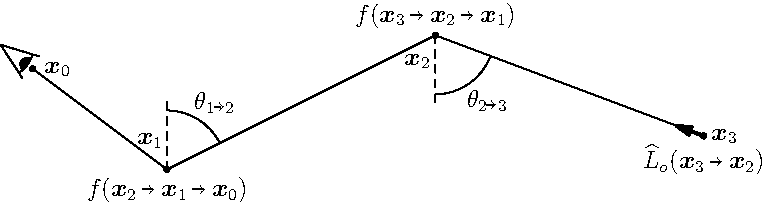
\includegraphics{asy/inference.pdf}
\caption{Visualization of the inference process.}
\label{fig:inference}
\end{figure}

Applying these observations to all path lengths up to termination, we get:
\begin{equation}
\label{eq:inference}
    I
    \hateq \sum_{i=1}^{n-1} T_i L_e(\pdir{i}{i-1}) + T_n \widehat{L}_o(\pdir{n}{n-1}), \quad
    T_n
    = \prod_{i=1}^{n} \frac{f(\ptrip{i-1}{i}{i+1}) \cos \theta_{i \veryshortarrow i+1}}{p(\pdir{i}{i+1} \mid \pdir{i-1}{i})}
\end{equation}
where $T_n$ is the accumulated throughput along the first $n$ segments of the path and $\widehat{L}_o(\pdir{n}{n-1})$ is the interpolated radiance estimate at the termination vertex.
To simplify notation, the path now starts at the eye vertex $\vec{x}_0$.
Note, that we do not have to divide by the path termination probability like we did in Russian Roulette Termination (\cref{eq:rr}), as we terminate the path with a valid radiance estimate.

To improve the quality of the inference pass, we can additionally apply Next Event Estimation with Multiple Importance Sampling like in the following section and the reference pathtracer.

\section{Path Tracing}
\label{sec:re_eye}
\begin{figure}[htb!]
    \centering
    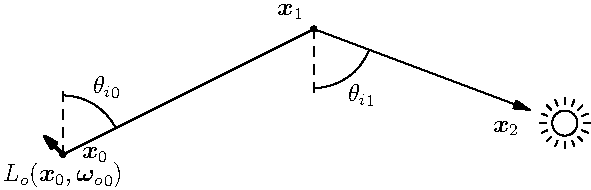
\includegraphics{asy/eye_tracing.pdf}
\caption{The simplest way to estimate the outgoing radiance $L_o(\x_0, \wo_0)$ is eye tracing, which shoots a path from the surface into the scene and collects emissions at each intersection.}
\label{fig:eye_tracing}
\end{figure}
We can apply the observations made in \cref{sec:inference} to the path space formulation for radiance (\cref{eq:path_space_integral_radiance}) to derive a path tracing based radiance estimator:
\begin{equation}
    L_o(\vec{x}_0, \wo_0)
    \hateq \sum_{k=1}^{\infty} T_k L_e(\vec{x}_k, \wo_k), \quad
    T_n
    = \prod_{k=0}^{n-1} \frac{f(\wi_k, \x_k, \wo_k) \cos {\theta_i}_k}{p(\wi_k \mid \wo_k)}
\end{equation}

\begin{figure}[htb!]
    \centering
    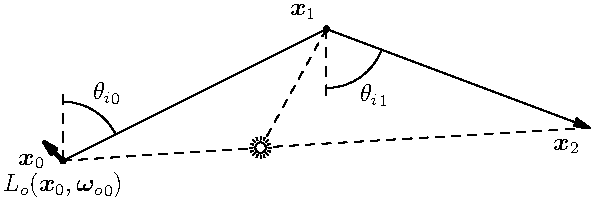
\includegraphics{asy/nee.pdf}
\caption{Direct light sampling also known as Next Event Estimation (NEE) performs significantly better than BSDF sampling on small direct lighting.}
\label{fig:nee}
\end{figure}
This estimator alone however is ineffective at finding small light sources, so we combine it with Next Event Estimation through Multiple Importance Sampling (\cref{sec:mis}), as we already did in the reference pathtracer:
\begin{equation}
\begin{aligned}
    L_o(\vec{x}_0, \wo_0)
    \hateq \sum_{k=1}^{\infty} T_k \left( w_\text{BSDF} L_e(\x_k, \wo_k) + w_\text{L} \frac{f(\pdir{L}{k}, \wo_k) \G{k}{L} L_e(\pdir{L}{k})}{p(\x_L)} \right)
\end{aligned}
\end{equation}
By combining the two techniques by weighting them with their respective MIS-weights $w_\text{BSDF}(\wo)$ and $w_\text{L}(\x_L)$ (\cref{eq:balance_heuristic} and \cref{eq:power_heuristic}), we get the best of both worlds.
For brevity, the parametrization of the MIS-weights is dropped in the equation above.
This combined with ReSTIR DI \parencite{bitterli2020} and a LightBVH \parencite{moreau2019} for efficient many light sampling is the radiance estimator used by \textcite{muller2021}.
Nevertheless, I simply sample the light source from a precomputed CDF-table by inversion sampling, because my test scenes only contain a few light sources.
To limit the path length, I use Russian Roulette Termination (\cref{eq:rr}) again, and in praxis the path length also has to be limited to a maximum length, which introduces potential bias.

\paragraph{Query Prediction}
In practice, I only predict queries by shooting primary camera rays, because this is already a good approximation of the query sampling distribution $Q(q)$ for the path termination strategies given in \cref{sec:path_termination}.
A more accurate and efficient method however would be to randomly draw queries from the queries already generated in the previous inference stage.
% TODO: Implement

\section{Bidirectional Training (BT)}
\label{sec:re_bidir}
\begin{figure}[htb!]
    \centering
    \begin{subfigure}{0.5\textwidth}
        \centering
        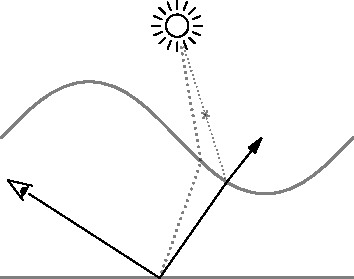
\includegraphics{asy/caustic.pdf}
        \caption{NEE}
        \label{fig:caustic_nee}
    \end{subfigure}%
    \begin{subfigure}{0.5\textwidth}
        \centering
        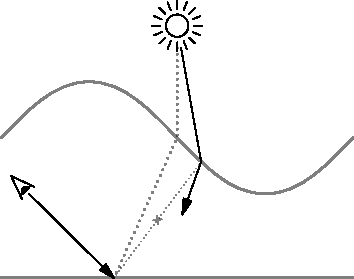
\includegraphics{asy/caustic_bidir.pdf}
        \caption{Reverse NEE}
        \label{fig:caustic_bidir}
    \end{subfigure}
    \caption{Caustics are difficult to capture with path tracing, since only a small fraction of the path space actually contributes to the caustic (dotted lines). NEE does not help, as most connecting samples will have zero contribution (crossed line) when the material is glossy.}
    \label{fig:caustic}
\end{figure}
A major weakness of the aforementioned radiance estimator (\cref{sec:re_eye}) is indirect lighting where the light paths undergo glossy reflections/refractions before getting diffused.
This effect is known as a caustic.
In the extreme case of an infinitesimal light source being ideally reflected/refracted and then diffused, path tracing and NEE even fail completely to capture this effect, because the probability to sample such a path by BSDF sampling is zero (\cref{fig:caustic_nee}). 
However, we can do the exact opposite of NEE by tracing light paths and connecting them to query points sampled from the eye.
This has the same problem as NEE for finding direct caustics (\cref{fig:caustic_bidir}), yet it discovers indirect illumination by caustics and long light paths very efficiently.

\begin{figure}[htb!]
    \centering
    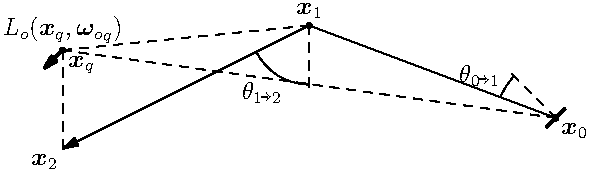
\includegraphics{asy/bidir.pdf}
    \caption{Flux is distributed along a BSDF-sampled path from a random point on a light source ($\x_0$). At the query point $\x_q$ radiance is collected by deterministically connecting to every vertex of the light path.}
    \label{fig:bidir}
\end{figure}
Specifically, I propose the following alternative radiance estimator based on this idea:
First, sample a query point $q = (\vec{x}_q, \wo_q)$ from the query sampling distribution $Q(q)$.
Then, trace a light path carrying flux from a randomly selected light source via BSDF sampling and connect each vertex $\vec{x}_k$ to the query point $\vec{x}_q$.

Starting again with a single-sample Monte Carlo Estimator for the Path Space Integral for Radiance (\cref{eq:path_space_integral_radiance}) and applying the same observations as in \cref{sec:inference}, we get:
\begin{equation}
\label{eq:bidir}
\begin{aligned}
    L_o(\vec{x}_q, \wo_q)
    &\hateq \frac{L_e(\pdir{0}{q})}{p(\x_0)} \G{0}{q} f(\pdir{0}{q}, \wo_q) \\
    &+ \sum_{k=1}^{\infty} \Phi_k \cdot \f{k-1}{k}{q} \G{k}{q} f(\pdir{k}{q}, \wo_q), \\
    \Phi_n &= \frac{L_e(\pdir{0}{q}) \cos \theta_{0 \veryshortarrow 1}}{p(\x_0) p(\pdir{0}{1})} \prod_{i=2}^{n} \frac{f(\ptrip{i-1}{i}{i+1}) \cos \theta_{i \veryshortarrow i+1}}{p(\pdir{i}{i+1} \mid \pdir{i-1}{i})},
\end{aligned}
\end{equation}
where $\Phi_n$ is the light flux transported along the path.
The sum over the path length is split into two parts because the first vertex $\vec{x}_0$ is sampled directly on the light source and requires special handling.

\section{Light Training (LT)}
\label{sec:lt}
\begin{figure}[htb!]
    \centering
    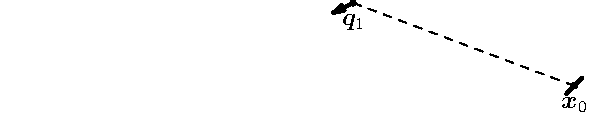
\includegraphics{asy/light_bootstrapping_1.pdf}
    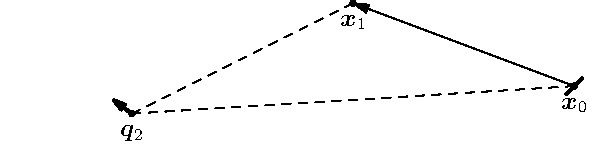
\includegraphics{asy/light_bootstrapping_2.pdf}
    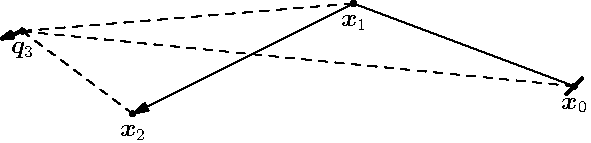
\includegraphics{asy/light_bootstrapping_3.pdf}
    \caption{Visualization of light training for query prediction: Every new light vertex is first handled as a query ($\vec{q}_i$) and collects radiance from all previous vertices according to \cref{eq:bidir}.}
    \label{fig:light_bootstrap}
\end{figure}
Despite sampling light paths, the estimator from \cref{sec:re_bidir} only finds indirect illumination by caustics efficiently, since given a specific query, the probability to connect to a glossy light path directly is still low (\cref{fig:caustic_bidir}).
So, instead of predicting queries solely from the eye, we can also collect radiance at future vertices of the light path (see \cref{fig:light_bootstrap}).
At a light vertex, we are guaranteed to get strong contribution at least from the previous vertex, because we sampled it directly through BSDF sampling.
It would also be possible to sample independent queries from the light vertices instead of reusing the next light vertex and this may in fact be an interesting algorithm to explore, though this is outside the scope of this thesis.

\begin{figure}[htb!]
    \centering
    \begin{subfigure}{0.5\textwidth}
        \centering
        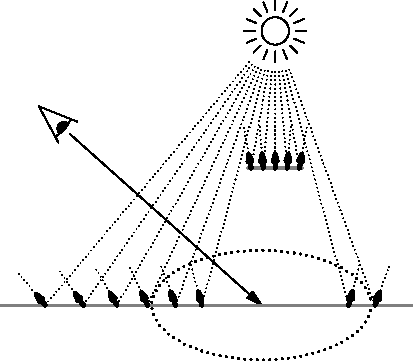
\includegraphics{asy/balancing.pdf}
        \caption{Shadows}
        \label{fig:balancing_shadows}
    \end{subfigure}%
    \begin{subfigure}{0.5\textwidth}
        \centering
        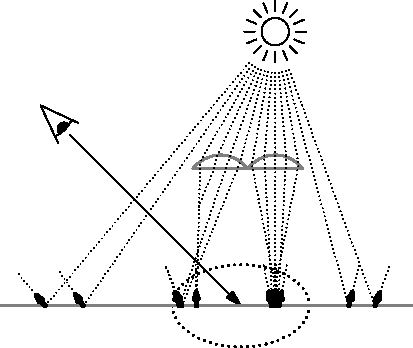
\includegraphics{asy/balancing_caustics.pdf}
        \caption{Caustics}
        \label{fig:balancing_caustics}
    \end{subfigure}
    \caption{Sources of bias in light training: The solid arrows indicate cache queries. In both cases, the interpolation should return zero radiance, as the points are not reached by light. However, since the cache is filled by light tracing, all available nearby estimates are lit, resulting in a bright prediction.}
    \label{fig:balancing}
\end{figure}

\paragraph{Balancing} Although this estimator may look promising at first, it is important to note that it exhibits the problem already discussed in my motivation of bidirectional radiance caching (\cref{par:cache_efficiency}):
By sampling queries solely from the light, queries that are shadowed will never be predicted, which introduces bias into the cache (see \cref{fig:balancing}).
This can be clearly visible depending on the scene and will be further discussed in the results chapter (\cref{chap:results}).

To counteract this drawback, we can make a simple observation:
If a query is not reachable from a light source, it does not receive energy, thus the radiance at such queries can be safely assumed to be zero.
Because the Neural Radiance Cache performs averaging in local neighborhoods, we can carefully introduce samples with radiance zero according to the query sampling distribution $Q(q)$.
By weighting the valid samples with the inverse of the ratio of valid samples, we can ensure that the mean over a local neighborhood is still correct:
\begin{equation}
\expectationvar{q}{{\widehat{L}_o}(\vec{x}_q, \wo_q)} = \frac{1}{n} \sum_{q \in Q} (1 - p_0) \cdot \frac{L_o(\vec{x}_q, \wo_q)}{(1 - p_0)} + p_0 \cdot 0 = \frac{1}{n} \sum_{q \in Q} L_o(\vec{x}_q, \wo_q)
\end{equation}

Essentially this algorithm models a sort of output decay on the NRC, dragging its prediction towards zero.
This can work, but it degrades the quality of the cache and makes training unstable, since it introduces additional noise with the zero radiance samples.
Furthermore, it is a waste of bandwidth to spend resources on learning zero radiance, as it does not provide any information gain.

\section{Sparse Progressive Photon Collection (SPPC)}
\label{sec:sppc}
The final radiance estimator I propose is an adaptation of Progressive Photon Mapping by \textcite{jensen1996,hachisuka2008}.
We again shoot flux into the scene by light tracing.
However, instead of collecting the flux by connecting to an infinitesimal query point, we collect the incoming flux over all sampled light paths in a \emph{query region} by kernel density estimation (see \cref{fig:pm_collection}).

The radiance at a query point $\x$ in direction $\wo$ can be estimated by:
\begin{subequations}
\label{eq:pm}
\begin{align}
    L_o(\x, \wo)
    &= \int_{\Omega_i} f(\wi, \x, \wo) L_i(\wi, \x) \cos{\theta_i} \diff\wi \label{eq:pm:lo}\\
    &= \int_{\Omega_i} f(\wi, \x, \wo) \frac{\diff^2 \Phi_i(\wi, \x)}{\diff A \; \cancel{\cos{\theta_i} \diff\wi}} \cancel{\cos{\theta_i} \diff\wi} \label{eq:pm:defrad}\\
    &\hateq \frac{1}{n} \sum_{k=1}^n f(\hat{\wi}_k, \x, \wo) \frac{\Delta \Phi_i(\hat{\wi}_k, \hat{\x}_k)}{\Delta A} w_{\vec{x}}(\hat{\x}_k)\label{eq:pm:est}\\
    &\approx \frac{1}{n \pi r^2} \sum_{k=1}^n f(\hat{\wi}_k, \x, \wo) \Delta \Phi_i(\hat{\wi}_k, \hat{\x}_k) w_{\vec{x},r}(\hat{\x}_k), \label{eq:pm:sphere}
\end{align}
\end{subequations}
where $w_{\vec{x},r}(\hat{\x}_k)$ is the kernel weight for the photon position $\hat{\x}_k$.
We start with the rendering equation (\cref{eq:pm:lo}) and replace the incoming radiance $L_i$ by its definition as incoming flux per area and solid angle (\cref{eq:pm:defrad}).
We then replace the integral by a Monte Carlo estimator over $n$ sampled flux packages \emph{(photons)} (\cref{eq:pm:est}).
Finally, we assume that the kernel function $w_{\vec{x},r}(\hat{\x}_k)$ is limited to a sphere of radius $r$.
Assuming the surface is locally flat, this allows us to approximate the surface area $\Delta A$ over which we are integrating by a disk of area $A=\pi r^2$ (\cref{eq:pm:sphere}).
The simplest such kernel function is the box function, with $w_{\vec{x},r}(\hat{\x}_k)=1$ inside the sphere and $0$ outside.
\begin{figure}[htb!]
    \centering
    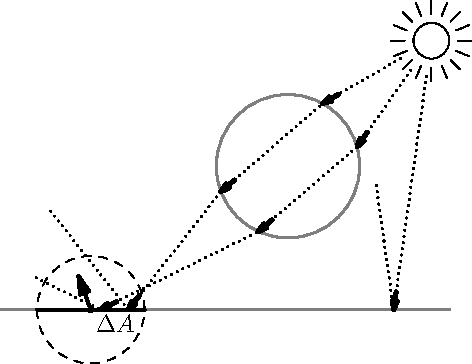
\includegraphics{asy/pm_collection.pdf}
    \caption{Visualization of photon mapping. Photons (packages of flux, here small black arrows) are distributed in the scene and collected over query regions (dashed circle). In this example, three light paths were sampled ($n=3$). Note, that in practice photons and queries are not recorded at glossy surfaces, since they probably can not be connected with high contribution. This removes glossy features from the radiance estimate, however the path termination strategies from \cref{sec:path_termination} avoid querying glossy surfaces in the first place.}
    \label{fig:pm_collection}
\end{figure}

\paragraph{Query Lifetimes}
Because we couple Photon Mapping with radiance caching, we can make some important modifications to the original algorithm:
Firstly, we do not need to query the photon map at every pixel, since the radiance cache interpolates between sparse samples.
So, we can reduce the amount of queries to a fixed number independent of render resolution.
Secondly, we can store the \emph{queries} instead of the \emph{photons} in a spatial data structure.
This enables the queries to persist across multiple frames and collect incoming flux over multiple light passes.
The lifetimes of the queries can be made completely independent of each other by keeping track of the total amount of light samples already drawn at creation time of a query.
The difference between the current count of light samples and the count at creation gives the number of total light samples $n$ that are used in the collection of flux for that query (\cref{eq:pm}).
Flux is simply accumulated to the query whenever a photon hits the query region.
To maintain a constant number of queries I use a ring buffer with an atomic index counter and a constant query replacement fraction $\kappa$.
The lifetime of a query is thus approximately $1/\kappa$ frames, yet it can also be longer if query prediction fails to produce a valid result, for example if a camera ray does not hit any geometry.

\begin{table}
    \centering
    \begin{subtable}{.45\textwidth}
        %\centering
        \caption{Photon}
        \label{tab:photon_struct}
        \begin{tabular}{l p{4cm}}
            %\toprule
            \textbf{Field} & \textbf{Description} \\
            \midrule
            $\x \in \mathbb{R}^3$ & Position \\
            $\wi \in \mathbb{S}^2$ & Incident direction \\
            $\Phi_i \in \mathbb{R}^3$ & Flux \\
            $\vec{n} \in \mathbb{S}^2$ & \emph{Surface normal for normal rejection (optional)} \\
            %\bottomrule
        \end{tabular}
    \end{subtable}%
    \begin{subtable}{.55\textwidth}
        %\centering
        \caption{Query}
        \label{tab:query_struct}
        \begin{tabular}{l p{5.5cm}}
            %\toprule
            \textbf{Field} & \textbf{Description} \\
            \midrule
            $\x \in \mathbb{R}^3$ & Position \\
            $\wo \in \mathbb{S}^2$ & Outgoing direction \\
            $\Phi_o \in \mathbb{R}^3$ & Accumulated outgoing flux \\
            $r \in \mathbb{R}$ & Radius \\
            $\vec{n} \in \mathbb{S}^2$ & Surface normal at $\x$ \\
            $f : \mathbb{S}^4 \to \mathbb{R}^3$ & BSDF at $\x$ \\
            $n_c \in \mathbb{N}$ & Number of total light samples at creation \\
            $N \in \mathbb{R}$ & Amount of photons collected in all passes \\
            $M \in \mathbb{N}$ & Number of photons collected in current pass \\
            %\bottomrule
        \end{tabular}
    \end{subtable}
    \caption{The structs used to represent photons and queries. Unit vector compression strategies \parencite{cigolle2014} could be applied to reduce the memory footprint. To keep the code simple however, this is not done in the accompanying implementation.}
\end{table}

\paragraph{Radius Reduction}
Choosing the radius $r$ is a trade-off between variance and bias.
Larger radii collect flux over a larger area, increasing the number of photons used in the estimator and thus reducing variance.
However, this also introduces bias, as these additional photons may not be an accurate representation of the incoming flux at the query point.
Shrinking the radius $r$ towards zero eliminates this bias in the limit, but the number of available estimates also decreases, increasing the variance.
More precisely, \textcite{knaus2011} showed that $\mathrm{Bias}\left[\estimator{{L_o}_\mathrm{PM}}\right] \sim r^2 \sim 1/\mathrm{Var}\left[\estimator{{L_o}_\mathrm{PM}}\right]$.

Leveraging this observation, \textcite{hachisuka2008} developed Progressive Photon Mapping (PPM), originally as a technique to make classic Photon Mapping consistent and to overcome the memory constraint of storing a single large photon map.
Their idea was to perform multiple light passes, shrinking the radius after each iteration, yet never too much, as there has to be a gain in the total amount of photons, otherwise the estimator diverges.
Therefore, they introduce a factor $\alpha$ to control the fraction of photons to keep after each light pass (\cref{eq:ppm_n}).
By fixing the photon density inside the area of the query (\cref{eq:ppm_r}), they derive following update rules:
\begin{subequations}
\begin{align}
    \text{Let } N' = N + \alpha M \label{eq:ppm_n}\\
    \frac{N + M}{A} = \frac{N + M}{\pi r^2} \stackrel{!}{=} \frac{N'}{\pi (r^2)'} = \frac{N'}{A'} \implies (r^2)' = r^2 \frac{N'}{N + M} \label{eq:ppm_r}\\
    \Phi_o' = \Phi_o \frac{A'}{A} = \Phi_o \frac{\pi (r^2)'}{\pi r^2} = \Phi_o \frac{N'}{N + M}, \label{eq:ppm_f}
\end{align}
\end{subequations}
where $N$ is the total amount of collected photons, $M$ is the number of new photons found during the light pass, and $r$ and $A$ are the respective radius and area of the query.
The total outgoing flux has also to be scaled down to the reduced area $A'$ (\cref{eq:ppm_f}).

\paragraph{Hardware Acceleration}
The original k-d-tree method of storing photons by \textcite{jensen1996} is not suitable for GPUs.
Thus, this implementation instead follows the idea of \textcite{evangelou2021}, who proposed to leverage hardware accelerated Bounding Volume Hierarchies (BVHs) for fast Fixed-Radius-Near-Neighbor queries.
Their approach is to store the queries as balls of radius equal to their search radius $r_i$ and to represent the data points by shooting infinitesimal rays.
Finding an intersection is then equivalent to finding a data point within $r_i$ around the query.

\paragraph{Algorithm Overview}
Applied to Photon Mapping, this means we first store the Axis-Aligned Bounding Boxes (AABBs) of the queries in an array and use OptiX to construct a BVH.
Then, we sample the light paths and at each non-specular scene intersection (\cref{par:pt_1st_diffuse}), we shoot infinitesimal rays into the query-BVH.
In the intersection program, we simply compare the squared distance to the ray origin with the squared radius of the query ball.
If the distance is smaller, we atomically accumulate the BSDF-weighted incoming flux of the photon to the flux of the query $\Phi_o$.
After the light pass we apply radius reduction and use the radiance estimates to update the radiance cache.

\paragraph{Notes on Performance}
If the queries are dense or the radius is large, many queries will overlap, causing the atomic accumulation to be serialized and stalling the GPU threads.
This is the reason why \textcite{kern2023} store the \emph{photons} instead of the queries in the BVH, which forces them however to use a global radius reduction scheme \parencite{knaus2011}.
Yet, because we allow the queries to have independent lifetimes, a global radius is not applicable in our case, rendering their approach incompatible.
Fortunately though, we partially avoid serialization since our queries are only distributed sparsely.
An interesting idea to resolve this problem would be to check for overlap during query prediction and reject queries that overlap too much with existing queries, or to use an iterative screen-space hole-filling approach like \textcite{stachowiak2018}.
This would also automatically sample caustics more densely, as caustics receive more light samples, making the radius shrink faster, thus reducing overlap and creating space for new queries.
Additionally, \textcite{kern2023} stochastically reject $70\%$ of all non-caustic photons, which could also benefit performance in our case.
Furthermore, to improve quality at corners, they reject photons with strongly deviating normals.

%\section{Hardware Accelerated Vertex Connection and Merging}